\documentclass[conference]{IEEEtran}
\IEEEoverridecommandlockouts
% The preceding line is only needed to identify funding in the first footnote. If that is unneeded, please comment it out.
\usepackage{cite}
\usepackage{amsmath,amssymb,amsfonts}
\usepackage{algorithmic}
\usepackage{graphicx}
\usepackage{textcomp}
\usepackage{xcolor}
\usepackage{minted}
\usepackage{array}
\usepackage{float}
\usepackage{multicol}
\def\BibTeX{{\rm B\kern-.05em{\sc i\kern-.025em b}\kern-.08em
    T\kern-.1667em\lower.7ex\hbox{E}\kern-.125emX}}
\begin{document}

\title{Image-Based Malware Classification Using Convolutional Neural Networks\\
}

\author{
\IEEEauthorblockN{Raymond Jiang}
\IEEEauthorblockA{\textit{Glen A. Wilson High School} \\
Hacienda Heights, United States \\
raymondjiang0917@gmail.com}
\and
\IEEEauthorblockN{Mohammad Husain}
\IEEEauthorblockA{\textit{Cal Poly Pomona} \\
\textit{Inaugural Director of the PolySec Cyber Lab}\\
Diamond Bar, United States \\
mihusain@cpp.edu}
}

\maketitle

\begin{abstract}
As the increasingly tech world becomes more and more integrated into our lives, so does the sophistication of malware. Effective malware classification is an important step for the prevention and mitigation of malware as it allows the identification of new threats without reliance on existing malware databases. Traditional techniques, such as manual code analysis, often have significant limitations and can be easily prevented by attackers. This paper proposes a novel approach to malware classification by directly analyzing the malware file itself, bypassing the need for code disassembly. By converting the malware bytes file into an image, this step completely skips the need to look through the actual code to identify it, rendering code obfuscation ineffective.  We employ a Convolution Neural Network (CNN) based architecture to classify each image, using its pattern recognition capabilities. Our approach demonstrates significant improvements in accurately detecting and classifying new malware threats. Our findings indicated that the use of an CNN model to classify malware types are accurate and are a more dependable way for classification, creating a future possibility to detect newly created malware and take prevention measures early on.
\end{abstract}

\begin{IEEEkeywords}
malware classification, code analysis, malware, Convolution Neural Network (CNN), code obfuscation
\end{IEEEkeywords}

\section{Introduction}
Since the creation of the internet, malicious code has been written to exploit software bugs and perform malicious tasks. The first ever malware written exploited the lack of security in a system called ARPANET.\cite{i1} However, in its most basic form, malware is just code written that, when executed, performs a specific task, which in most cases is meant for harm.\cite{i2} While software developers are patching these exploits, it becomes a problem when these exploits are found before such developers. This presents the issue of Zero-Day exploits\cite{i3}, allowing attackers to use custom and never-before-seen malware. There are several ways to classify malware; however, each has flaws.

The most common way is code analysis, which involves manually reviewing each malware's code. To start this process, the malware file would often need to decompile the malware file using various applications to access its original code. Similarly, there is static code analysis, in which instead of a human going through code line by line, a program goes through it and identifies possible vulnerabilities in it.\cite{i4} However, this type of analysis can be prevented by code obfuscation, which can prevent disassembles or humans from reading clear code.

Current antivirus programs also use signature-based detection as one of their main lines of defense against malware. Signature-based detection scans through every file signature or a file's information.\cite{i5} It will then match it to a vast database of known malware signatures and determine if it should be blocked from the system. This approach is most commonly used and very effective for various reasons. Its efficiency is unrivaled by other techniques due to its simplicity; it is only a matching system that checks if a particular file is in its malware database. Since it only matches and does not make predictions, this system is highly accurate, making it a trustworthy technique. However, due to its structure, it has a few limitations. Since it only matches malware to a database, the new malware created will only be detected once registered. On top of that, constant updates are required to keep up with the new malware types. 

The technique we will attempt to employ is similar to signature-based detection but without its limitations. We will be training an AI Convolutional Neural Network\cite{i6} to identify malware files. By doing this, our goal is to be able to classify malware whose code is not obfuscated, eliminating the limitation presented by static code analysis. On top of this, by using the CNN model to classify malware, we plan to train on previous databases of malware similar to one of signature-based detection. However, on top of being fed known malware, the model can also make predictions for the future, including new malware based on what they have seen before. This allows this model to fill for the lack of predictability in signature-based detection and could also be combined with it to fill the roles of both accuracy and future predictability.

\section{Related Works}
This section provides a comprehensive overview of previous research, encompassing different classification techniques mainly regarding using machine learning models as the basis for classification. These studies have contributed heavily into various domains of experimentation including but not limited by: Android, Windows, etc.

    H. AlOmari \textit{et al}  \cite{r1}  investigates the performance of different machine learning algorithms in detecting various Android-based malware using the CICMalDroid2020 dataset comprised of 11,598 APKs. They used CopperDroid to use dynamic feature extraction on each APK. They preprocessed the data using Synthetic Minority Oversampling Technique (SMOTE) and normalized values via Z-score normalization in preparation for the model. They used various machine learning classifiers such as LightGBM, Random Forest, Extra Trees, Gradient Boosting, Decision Trees, K Neighbors, and Ada Boost in their evaluation. Their results found that the Light Gradient Boosting Machine (LightGBM) algorithm was the most effective, having an F1-score of 94.77\%. The authors have also found that data preprocessing steps, such as data normalization, significantly improved the performance of Logistic Regression. Similarly, SMOTE dealt with class imbalance, which improved the performance of many classifiers.

    A. Wajid \textit{et al} \cite{r2}  explores the different techniques used for code analysis: static, dynamic, and hybrid, using data from previous research papers. The authors compare signature-based analysis (static) and behavior-based analysis (dynamic). Their data comes from papers within the following criteria: relevance, publication year, data validity, methodology, and evaluation. They want their selected papers to be relevant to malware detection using machine learning models in Windows, they must be published between 2019 - 2023 to be updated enough, the data used in the experiment must be publically available, the experiments in each paper must use machine learning algorithms, and finally, the results of the study must be quantifiable using standard metrics like accuracy. From what they saw from their collected articles, it can be seen that the Random Forest machine learning model is the most consistent, with accuracy rates varying from 98.63\% to 99.8\%. They also separated these articles into either feature-based or image-based approaches. Feature-based methods extract data from malware binaries, such as PE headers, API calls, opcode sequences, etc., for classification. In contrast, image-based methods convert the malware binary files into images (greyscale or RGB) and use image classification machine learning models. They found that static analysis was often much faster and safer, as it required no actual execution of the file, only looking at the code. However, it had limitations that dynamic analysis picked up on; it could often be prevented via code encryption or other forms of obfuscation, and it could also not observe runtime interactions of the malware. On the other hand, dynamic analysis filled up the flaws left by static analysis; it required the actual execution of the code in a controlled environment. This allowed models to pick up on its actions and also allowed it to predict and identify new malware types. However, its limitations would be that it was very computationally heavy, as it required running each malware file in a sandbox, which can be time-consuming. They proposed using a hybrid analysis technique, incorporating the pros from each type of analysis and combining them. 

    H. S. Anderson \textit{et al} \cite{r3}  introduced their dataset called EMBER, an open dataset for machine learning models used regarding Windows malware, specifically portable executable files. This dataset contains approximately 1.1 million data lines split with an 82 to 18 training-to-testing data ratio. The 900,000 training samples are split between 300,000 malicious, 300,000 benign or harmless, and 300,000 unlabeled data. The 200,000 testing samples were split into a 50:50 ratio of 100,000 malicious and 100,000 harmless. The data is a collection of JSON lines, in which each line or object contains data about each malware. The format includes sha256, date, label, and raw features. The sha256 contains the sha256 hash of the specific malware file; the date is the estimated date that the malware was first seen, and the label is used to define if the file is malicious, benign, or unlabeled. Their goal for this paper was to contribute to the cyber security industry by providing a massive and open dataset to increase more data within the domain. They built a decision tree baseline model based on LightGBM fed with the EMBER dataset to test the dataset. The model was a gradient-boosted decision tree (GBDT) trained using LightGBM with only default parameters. The results of this model were very promising; it received a high ROC AUC score (0.99821), indicating that it could classify the testing data well. This was compared with MalConv, a deep learning machine learning model with hyper-parameter optimization. This comparison noted that the baseline model trained solely using the EMBER dataset outperformed MalConv. 

    P. Maniriho\textit{ et al} \cite{r4}  conducted a systematic literature review on Windows malware detection techniques. They focused on static, dynamic, and hybrid analysis methods that these articles used as their results. They identified two methods of static analysis: signature-based detection and heuristic-based detection. Signature-based detection relies on an extensive database of malware signatures and uses it to identify existing malware. On the other hand, heuristic-based detection looks at code patterns to check for potential malicious behavior. In the case of dynamic analysis, they have defined it in two categories: behavior-based detection and memory analysis. Behavior-based detection runs the malware program in a controlled system and analyzes its behavior to detect zero-day vulnerabilities. Memory analysis uses dumps to find the program's activities and detect if they are malicious. The third and last technique they reviewed would combine the previous two, called hybrid analysis. Both are combined to improve accuracy through each technique's strengths. The paper mentions primary datasets such as CSDMC2010, MalImg, Microsft BIG2015, and EMBER, which were all essential in evaluating malware detection techniques in their reviewed papers. These public datasets allow others to reproduce and scale their programs. They also looked at biases that could have affected performance, such as temporal, spatial, and sample size. These biases are essential to consider since they can vastly change an experiment's results and make them less reliable if too large. When measuring the performance of each study's results, they often used standard performance metrics such as accuracy, precision, recall, F1 scores, and AUCROC scores. These scores can show each model's faults and be used to detect them. False negatives and false positives can be harmful in practice, producing skewed or incorrect results. This review provides information on the current and future states of malware detection in Windows, as presented in various studies.

\section{Methodology}

\subsection{The Dataset}
    The data used to train and test the convolutional neural network (CNN) were from the malimg dataset\cite{m1}  which consists of 9,339 malware images from 25 different classes.
    
\begin{figure}[htbp]
\centerline{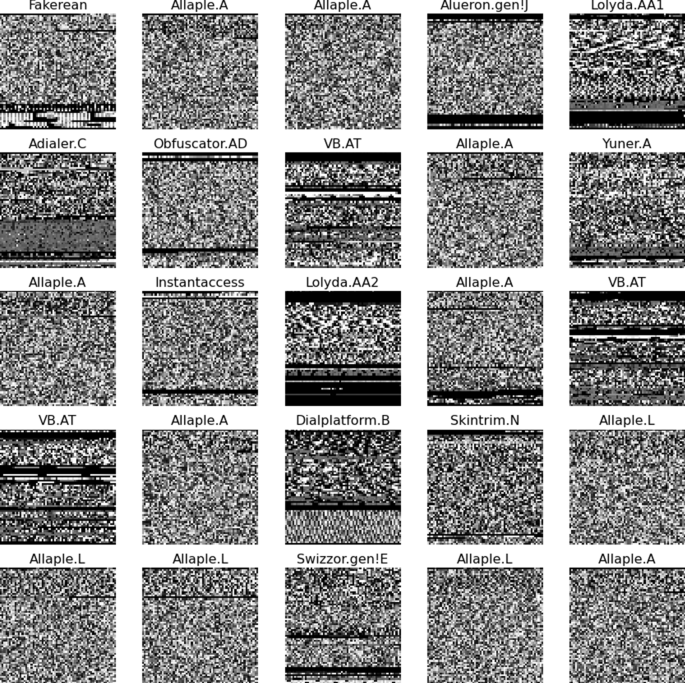
\includegraphics[width=1\linewidth]{images/malImg dataset picture.png}}
\caption{Sample pictures of the malImg dataset from each of the 25 different malware families.}
\label{fig}
\end{figure}
The classes included:
\begin{multicols}{2}
\begin{itemize}
    \item VB.AT
    \item Yuner.A
    \item Swizzor.gen!E
    \item Swizzor.gen!I
    \item Wintrim.BX
    \item Rbot!gen
    \item Lolyda.AA1
    \item Lolda.AA2
    \item Lolyda.AT
    \item Instantaccess
    \item Skintrim.N
    \item Obfuscator.AD
\end{itemize}
\columnbreak
\begin{itemize}
    \item Lolyda.AA3
    \item Fakerean
    \item Malex.gen!J
    \item Alueron.gen!J
    \item C2LOP.gen!g
    \item Allaple.A
    \item C2LOP.P
    \item Dontovo.A
    \item Allaple.L
    \item Adialer.C
    \item Dialplatform.B
    \item Autorun.K
    \item Agent.FYI
\end{itemize}
\end{multicols}
\subsection{Data Preprocessing}
When presented with such a large dataset, filtering out data and processing it is a essential step in making sure a model is trained properly.  In our case, we used keras's built in preprocessing class called ImageDataGenerator().

Since we were importing from a folder,  we would use the method flow\_from\_directory, which ended up looking like this: ImageDataGenerator().flow\_from\_directory(root, target\_size=(64,64), batch\_size=10000)

\begin{table}[htbp]
\caption{Parameters for Preprocessing}
\begin{center}
\begin{tabular}{|>{\centering\arraybackslash}p{0.15\linewidth}|>{\centering\arraybackslash}p{0.8\linewidth}|}
\hline
\textbf{Parameter}&\textbf{Details}\\ \hline 
root& Specifies the directory of the folder containing classes\\
\hline
target\_size& The size of each image in pixels; in our case, each image was 64 x 64 \\\hline
 batch\_size& The amount of images to be processed; in our case there were 9339 images, so a batch size of 10,000 would be able to load all images\\\hline\end{tabular}
\label{m1}
\end{center}
\end{table}
We would then use the next() function to iterate through the array of images, separating data into two numpy arrays, one for the image itself, and the other for its class/label name. This is done so that each element in the image corresponds for to the same element in the same index of the label array.
\\\\
The result would be two arrays with a total of 9339 data indexes in each:\\
images.shape = (9339, 64, 64, 3)
    \begin{itemize}
  \item 9339 total images
  \item 64 by 64 is the size of each image
  \item  3 colors are used (Red, Green Blue)
\end{itemize}
labels.shape = (9339, 25)
\begin{itemize}
  \item 9339 total images with labels
  \item 25 different labels in total\\
\end{itemize}
Our final step to processing data would be to split data up in to proper proportions for model training. In this step, we opted to use a 70:30 training to testing ratio, making use of keras's train\_test\_split() method. This creates for us 4 different arrays, similar to images and labels from above but split into training and testing.

\begin{table}[htbp]
\caption{Preprocessing Results}
\begin{center}
\begin{tabular}{|c|c|}
\hline
\textbf{Array}&\textbf{Details}\\ \hline 
X\_train& Array of images for training\\
\hline
X\_test& Array of images for testing\\\hline
 Y\_train& Array of labels for training\\\hline
 Y\_test&Array of labels for training\\\hline\end{tabular}
\label{m2}
\end{center}
\end{table}

This ended with 6537 data values for training and 2802 for testing
\newpage
\subsection{Model Structures}
This section takes a look at the various structures/layers of the convolutional neural network model used for testing, and the an overall look of each structure's purpose.

\begin{table}[htbp]
\caption{CNN Layers}
\begin{center}
\begin{tabular}{|c|>{\centering\arraybackslash}p{0.6\linewidth}|}
\hline
\textbf{Layer Name}  &\textbf{Layer Details}\\ \hline 
Input & Instantiates a Keras tensor from input\\
\hline
Conv2D & Applies convolutional filters to extract features from input\\\hline
 MaxPooling2D& Reduces dimensions by taking the maximum value over a grid of values\\\hline
 BatchNormalization& Normalizes inputs\\\hline
 Flatten& Converts multidimensional tensor into a single vector\\\hline
 Dense& Used for training and making predictions through interconnnected nodes\\\hline
 Dropout& Randomly drops nodes during training to prevent overfitting\\\hline\end{tabular}
\label{tab1}
\end{center}
\end{table}
Using these layers, there were three iterations of structures before we found the most optimal version, a model that didn't over fit nor under fit. Under fitting would mean that the model was unable to properly train, with a low accuracy rate during both the training and testing.\cite{m5} On the other hand, over fitting is the opposite, the model is so close to the training data the new testing data results in large drops in prediction accuracy.\cite{m4}\\

\subsubsection{Starter Model}
With this model, we used the following structure:
\begin{table}[H]
\caption{Starter Model Layers/Settings}
\begin{center}
\begin{tabular}{|c|>{\centering\arraybackslash}p{0.6\linewidth}|}
\hline
\textbf{Layer Name}  &\textbf{Layer Parameters}\\ \hline 
Input & (shape=(64, 64, 3))\\
\hline
Conv2D & (32, (3, 3), activation='relu', padding='same')\\\hline
 MaxPooling2D& ((2, 2))\\\hline
 BatchNormalization& NA\\\hline
 Flatten& NA\\\hline
 Dense& (128, activation='relu')\\\hline
 Dropout& (0.5)\\\hline
 Dense&(25, activation='softmax')\\\hline
 model.compile&(optimizer='adam', loss='categorical\_crossentropy', metrics=['accuracy'])\\\hline
 model.fit&(X\_train, Y\_train, epochs=20, batch\_size=64, validation\_data=(X\_test, Y\_test))\\\hline\end{tabular}
\label{tab1}
\end{center}
\end{table}

With this model, it was to be a starting point for us to try to find the most optimal parameters for each layer.  We would start off with the standard values for layers, such as 32 nodes for convolution2d, 128 node dense layer, and a 50\% dropout percentage. The activation functions used were also very standard, with RELU\cite{m2} used most of the time and SOFTMAX\cite{m3} used for the ending result layer. We had trialed this model and found out that 20 epochs is just enough for the model to develop and prevent overfitting, but also long enough to produce results accurately.\\

\subsubsection{Revised Model}

After solidifying working features of the starting model, we started to increase and change around values in the layers. With this model, we used the following structure:
\begin{table}[H]
\caption{Revised Model Layers/Settings}
\begin{center}
\begin{tabular}{|c|>{\centering\arraybackslash}p{0.6\linewidth}|}
\hline
\textbf{Layer Name}  &\textbf{Layer Parameters}\\ \hline 
Input & (shape=(64, 64, 3))\\
\hline
Conv2D & (32, (3, 3), activation='relu', padding='same')\\ \hline 
 MaxPooling2D&((2, 2))\\ \hline 
 BatchNormalization&NA\\\hline
 Conv2D &(64, (3, 3), activation='relu', padding='same')\\ \hline 
 MaxPooling2D&((2, 2))\\ \hline 
 BatchNormalization&NA\\ \hline 
 Conv2D &(128, (3, 3), activation='relu', padding='same')\\\hline
 MaxPooling2D& ((2, 2))\\\hline
 BatchNormalization& NA\\\hline
 Flatten& NA\\\hline
 Dense& (128, activation='relu')\\\hline
 Dropout& (0.5)\\ \hline 
 Dense&(128, activation='relu')
\\\hline
 Dropout&(0.5)\\\hline
 Dense&(25, activation='softmax')\\\hline
 model.compile&(optimizer='adam', loss='categorical\_crossentropy', metrics=['accuracy'])\\\hline
 model.fit&(X\_train, Y\_train, epochs=20, batch\_size=64, validation\_data=(X\_test, Y\_test))\\\hline\end{tabular}
\label{tab1}
\end{center}
\end{table}

With this model, our goal was to exaggerate as much as we could for the parameters and layers. We added 2 more sets of convolutional layers, each with twice more than the previous amount of nodes (32, 64, 128). In addition, we also added another dense layer with the same number of nodes (128) along with its same dropout percentage (50\%). We kept the same parameters for model compilation and fitting, both with adam optimizer and 20 epochs.\\

\subsubsection{Final Model}

With the revised model telling us the results of an extreme structure, we opted to find the middle ground between the starter and the revised model. With this model, we used the following structure:
\begin{table}[H]
\caption{Final Model Layers/Settings}
\begin{center}
\begin{tabular}{|c|>{\centering\arraybackslash}p{0.6\linewidth}|}
\hline
\textbf{Layer Name}  &\textbf{Layer Parameters}\\ \hline 
Input & (shape=(64, 64, 3))\\
\hline
Conv2D & (32, (3, 3), activation='relu', padding='same')\\ \hline 
 MaxPooling2D&((2, 2))\\ \hline 
 BatchNormalization&NA\\\hline
 Conv2D &(32, (3, 3), activation='relu', padding='same')\\ \hline 
 MaxPooling2D&((2, 2))\\ \hline 
 BatchNormalization&NA\\\hline
 Flatten& NA\\\hline
 Dense& (128, activation='relu')\\\hline
 Dropout& (0.5)\\ \hline 
 Dense&(128, activation='relu')
\\\hline
 Dropout&(0.5)\\\hline
 Dense&(25, activation='softmax')\\\hline
 model.compile&(optimizer='adam', loss='categorical\_crossentropy', metrics=['accuracy'])\\\hline
 model.fit&(X\_train, Y\_train, epochs=20, batch\_size=64, validation\_data=(X\_test, Y\_test))\\\hline\end{tabular}
\label{tab1}
\end{center}
\end{table}
With this model, we tried to find the middle ground between the previous models. I opted to use 2 convolution layers, each remaining with 32 nodes.  Two dense layers were kept, each with 128 nodes and an RELU\cite{m2} activation, paired with dropout layers of 50\%. We kept the same parameters for model compilation and fitting, both with adam optimizer and 20 epochs.


\begin{thebibliography}{00}
\bibitem{i1}Johanna, “The history of malware - Advenica,” Advenica, Apr. 11, 2024. https://advenica.com/learning-center/blog/the-history-of-malware/
\bibitem{i2}“The future of ransomware: Inside Cisco Talos threat hunters,” Cisco. May 16, 2024. [Online]. Available: https://www.cisco.com/site/us/en/learn/topics/security/what-is-malware.html
\bibitem{i3}“What is a Zero-Day Exploit? | IBM.” https://www.ibm.com/topics/zero-day
\bibitem{i4}“Static Code Analysis | OWASP Foundation.” https://owasp.org/www-community/controls/Static\_Code\_Analysis
\bibitem{i5}“What is Signature-Based Detection? | Corelight.” https://corelight.com/resources/glossary/signature-based-detection
\bibitem{i6}“What are Convolutional Neural Networks? | IBM.” https://www.ibm.com/topics/convolutional-neural-networks

\bibitem{r1}H. AlOmari, Q. M. Yaseen, and M. A. Al-Betar, “A Comparative analysis of machine learning Algorithms for Android Malware Detection,” Procedia Computer Science, vol. 220, pp. 763–768, Jan. 2023, doi: 10.1016/j.procs.2023.03.101.
\bibitem{r2}A. Wajid, T. Ahmed, and U. B. Chaudhry, “A comprehensive review of Machine Learning-Based Malware detection techniques for Windows Platform,” May 07, 2024. http://thenucleuspak.org.pk/index.php/Nucleus/article/view/1349
\bibitem{r3}H. S. Anderson and P. Roth, “EMBER: an open dataset for training static PE malware Machine learning Models,” arXiv.org, Apr. 12, 2018. https://arxiv.org/abs/1804.04637
\bibitem{r4}P. Maniriho, A. N. Mahmood, and M. J. M. Chowdhury, “A systematic literature review on Windows malware detection: Techniques, research issues, and future directions,” Journal of Systems and Software/the Journal of Systems and Software, vol. 209, p. 111921, Mar. 2024, doi: 10.1016/j.jss.2023.111921.

\bibitem{m1}“Papers with Code - Malimg Dataset.” https://paperswithcode.com/dataset/malimg
\bibitem{m2}B. Krishnamurthy, “An introduction to the RELU activation function,” \textit{Built In}, Feb. 26, 2024. https://builtin.com/machine-learning/relu-activation-function
\bibitem{m3}T. Wood, “Softmax Function,” \textit{DeepAI}, Jun. 25, 2020. https://deepai.org/machine-learning-glossary-and-terms/softmax-layer
\bibitem{m4}“What is Overfitting? | IBM.” https://www.ibm.com/topics/overfitting
\bibitem{m5}“What is underfitting? | IBM.” https://www.ibm.com/topics/underfitting
\end{thebibliography}

\end{document}
